% NOTE: Dr. Statman was going to show me a cool experiment with photo refractives.

% Abstract: Brief summary (one paragraph) of the paper. Terse.

% Introduction: give an overview of your work. In this section, describe the physics behind the experiments. This, in part, will be a regurgitation of what you've learned from the optics textbook. But in your own words, in your own order, and with elaboration based on what you've learned. Your point of view should be that the ultimate goal was to make vector holograms (even if it is still not clear what they are). So you should write this with that in mind.

% Experiment: This should be a simple description of your experiments with schematics. Explain, in words, what you did, what you tried that didn't work, what you tried that did work. Keep it simple, but include the various roadblocks. This should be a good reference if you were to continue the project in the fall.

% Results and Discussion: A simple discussion of your results and what you learned. Keep the level high and professional. This is not a high school lab report. You should include a paragraph on what you see as future work. I want to see that you are thinking of where one goes with this. It can be future work that you might want to pursue, but it doesn't have to be that limiting.

% References: Not a lot here.

% Remember, the paper is documentation of your work. But you also want to demonstrate that you are thinking beyond these experiments. Be creative! Have fun with it, but keep it professional. Don't worry about your grade. You've done well. Instead, write it with you in mind. Think, if you were to look at the paper your senior year, will you feel good about the quality of work presented your first year, or will you be embarrassed?

% DS

\documentclass[12pt]{article}
\usepackage[notes, backend=biber, isbn=false, doi=false, noibid]{biblatex-chicago}
\usepackage{wrapfig,graphicx}
\usepackage[letterpaper, left=2.5cm, right=2.5cm, top=1.8cm, bottom=.7cm]{geometry}
\usepackage{fancyhdr}
\usepackage{setspace}
\usepackage{amsmath}
\setstretch{1.20}
\bibliography{sources}
\graphicspath{ {./images/} }

\pagestyle{fancy}
\fancyhf{}
\rhead{\thepage}
\lhead{Allegheny College Department of Physics}

\begin{document}

\begin{center}
  \large Spring 2021 Independent Study

  \normalsize Simon Jones

  \footnotesize under Dr. David Statman
\end{center}
\vspace{-15px}
\noindent
\subsection*{Abstract}
This independent study focused on optics, the study of light. Through readings and numerous experiments familiarizing myself with optical instruments, I ended the year with an experiential understanding of optics, constructing a vector hologram, while being asynchronously introduced to it in my introductory electromagnetism course. Each Wednesday of the semester, Dr. Statman would assign a small task or experiment. The following day, I would spend roughly five hours conducting and documenting my assigned activity. In this document I outline my work, including the physics involved and the mistakes made.

\subsection*{Introduction}
There were many steps involved in bringing me to the point where I could conduct experiments; through readings and `tinkering' with instruments, I steadily became equipped enough to do so. The experimentation readied me to attempt to construct a vector hologram by the end of the semester.

I began the semester reading \textit{Introduction to Optics} by Pedrotti \autocite{pedrotti} to expose myself to terminology and equations used in optics. This started with the nature of light, where properties such as wavelength and frequency were discussed, going on to production and measurement of light, where radiometric and photometric quantities and equations such as luminous energy, flux, and exitance were discussed. Following this was an introduction to geometrical optics, which outlined the Law of Reflection,
\[\theta_a=\theta_b\]
explaining that the incident angle of a ray of light is equal to the reflected angle; Snell's Law,
\[n_a\sin{\theta_a}=n_b\sin{\theta_b}\]
showing that the $\sin$ of the incident is directly proportional to that of the reflected; and, more notable, the mirror or lens maker's equation,
\begin{equation}\label{lensmakers}
\frac{1}{s}+\frac{1}{s'}=\frac{1}{f}
\end{equation}
showing that the sum of the inverse object and image distances equals the inverse of the focal length of a lens or mirror. \autocite[1-61]{pedrotti}

% --------------------------------------------------------------
\vspace{15px}
\noindent
\large{\textbf{\S}} The first experiment of the semester involved me determining the polarization of a 488nm laser. This involved using a half waveplate, which phase shifts a component of the polarized laser beam by $\Delta\theta=\pi$. Effectively, the polarized laser's wave components are projected onto the axes of the half waveplate, which has a `fast axis' and a `slow axis'. The component projected onto the slow axis would interfere with the material of the waveplate, resulting in a phase shift, while the component projected onto the fast axis remains in phase. Recombining these modified components results a wave with a polarization flipped across the fast axis.

% --------------------------------------------------------------
\vspace{15px}
\noindent
\large{\textbf{\S}} Furthering the use of waveplates, the following experiment's objective was to determine the purpose of a quarter waveplate, which, similarly but not identically to the half waveplate, phase shifts a component of the polarized laser beam by $\Delta\theta=\frac{\pi}{2}$. The interesting thing about this waveplate is that the phase shift produces components whose resultant vectors follow a helical pattern as the wave propagates through space. When the phase shift is at its maximum, meaning equal slow and fast axis components are maintained, the elliptical pattern has an eccentricity of 0 producing circularly polarized light.

% --------------------------------------------------------------
\vspace{15px}
\noindent
\large{\textbf{\S}} To gain experience with lenses and geometrical optics, I set up a beam expander. A beam expander works by diverging a beam to then converge it to be parallel once it has reached a certain expansion. This produces a projected image from the resulting parallel beams. If the focal lengths of the lenses are aligned, the magnification is the ratio of the focal lengths,
\begin{equation}\label{magnification}
m=\frac{f_2}{f_1}
\end{equation}
This can be derived from the Eq.~\eqref{lensmakers}, taking into account each lens's respective image and object distance.

% --------------------------------------------------------------
\vspace{15px}
\noindent
\large{\textbf{\S}} Young's Double Slit Experiment is an experiment demonstrating destructive and constructive interference of polarized light in the form of fringe lines, vertical lines of alternating intensity projected onto a screen. The experiment can yield information about various properties of the laser passed through it. I was actually able to use it to calculate the wavelength of the laser!

By passing a beam of light through two thin, vertical slits a distance $a$ apart, each pair of rays pointing to a concentric point on the screen a distance $s$ away will differ in length by $\delta=a\sin\theta$, where $\theta$ is the angle of the ray from the optical axis. As each ray travels from its slit, its respective path length will differ from the other ray, which creates a phase shift. This phase shift will produce either constructive or destructive interference. We can also look at this phase shift as a distance measured in units of wavelength,
\begin{equation}\label{pathlengthdiff}
\delta=a\sin\theta=n\lambda
\end{equation}
When $\theta$ is small, we can say that $\sin\theta\approx\tan\theta$ which means that $\sin\theta\approx\frac{\Delta{y}}{s}$. Where $\Delta{y}$ is the distance between the first fringe line and the optical axis or $n=1$. Thus, plugging in Eq.~\eqref{pathlengthdiff},
\begin{equation}\label{wavelengthslitapprox}
\lambda\approx{a}\frac{\Delta{y}}{s}
\end{equation}
Note that $\Delta{y}$ remains constant for each wavelength the paths are separated by, so we could technically write Eq.~\eqref{wavelengthslitapprox} as $n\lambda\approx{a}\frac{\Delta{y}}{s}$. Using Eq.~\eqref{wavelengthslitapprox}, plotting $\frac{\Delta{y}}{s}$ versus $a^{-1}$ yields the wavelength as the slope, which we find is very helpful!

% --------------------------------------------------------------
\vspace{15px}
\noindent
\large{\textbf{\S}} Having familiarized myself with interference, I moved on to interfere two circularly polarized beams. Circularly polarized interference between right and left hand polarized light produces no visual difference in intensity because the beams only interfere with each other on a portion of each of their elliptical patterns; however, passing the interfered beams through a linear polarizer filters out the other polarizations of light to produce fringe lines that transform as the polarizer is rotated.

% --------------------------------------------------------------
\vspace{15px}
\noindent
\large{\textbf{\S}} To apply the culmination of my experience, Dr. Statman put me to work on creating a vector hologram. By passing right-left interfered light through a liquid crystal, the molecular structure of the liquid crystal would change such that, when passing a vertically polarized beam in the opposite direction through the liquid crystal, a row of dots will be visible on a screen from the vertically polarized beam passing through the molecular structure imposed by the interfered beams.

\subsection*{Experiments}
I will now outline my own personal experience, including my mistakes, in conducting these experiments.

% --------------------------------------------------------------
\noindent
\begin{wrapfigure}{r}{0.33\textwidth}
  \begin{center}
    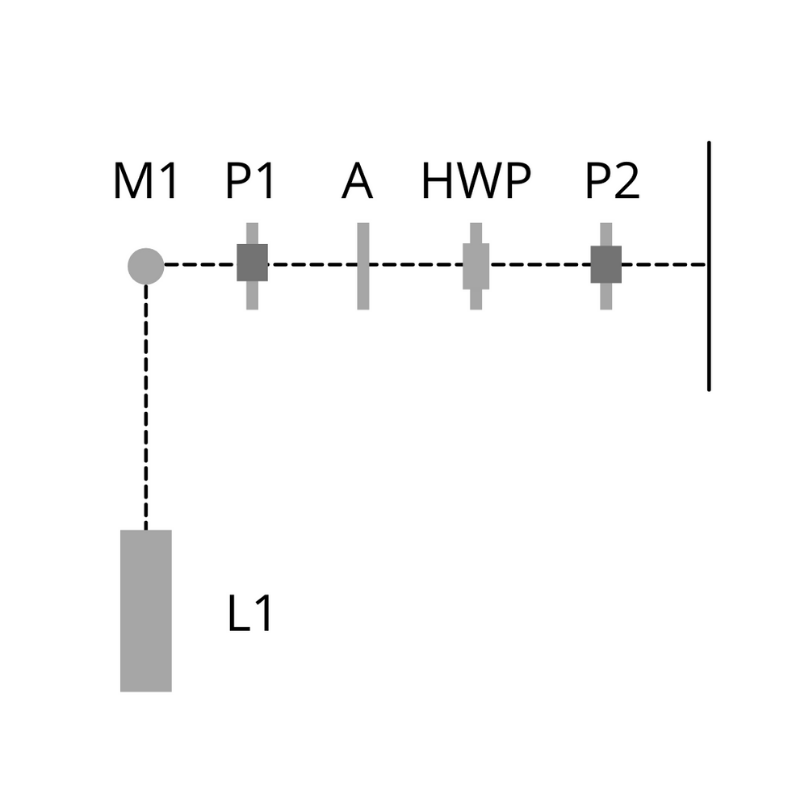
\includegraphics[width=0.31\textwidth]{E1}
  \end{center}
  \caption{Polarizers surrounding an aperture and a half waveplate. L1: laser, M1: mirror, P1: polarizer, A: aperture, HWP: half waveplate, P2: polarizer.}\label{E1}
\end{wrapfigure}
\large{\textbf{\S}}
My objectives in the first experiment were to find the polarization of the laser and to find what the half waveplate does. My setup, depicted in Fig.~\ref{E1}, had a laser reflected by mirror M1 entering polarizer P1, aperture A, half waveplate HWP, and polarizer P2, then projected onto a wall. This setup was already configured prior to our entering the lab, presumably by students from the previous semester. Initially, I struggled in grasping the concept of polarized light, but after seeing the changes in intensity as I rotated each polarizer, it was reified in my head. In finding the polarization of the light, I guessed that the light was polarized in the direction I saw a diffracted horizontal line in the far field of the wall; however, this was not the case. This was just a product of light reflecting off of scratches in the instruments. Once I noticed that the light would drop in intensity every $90^{\circ}$ I rotated the polarizer, I hypothesized that the light was polarized perpendicular to the orientation of the polarizer. Tracing the estimated polarization back through M1, I concluded that the polarization was vertical; Dr. Statman confirmed this conclusion.

The next step was the find out what the half waveplate did. I aimlessly rotated both both polarizers and the HWP, seeing periodic decreases in intensity without noticing any pattern. To narrow down the variables, I turned P1 horizontal (the light was horizontally polarized after passing through M1), P2 vertical, and only rotated the HWP. Normally, no light would be visible if horizontally polarized light passed through a vertical polarizer, but, upon rotating the HWP every $90^{\circ}$, the intensity would increase to a maximum. I was able to conclude that indeed, the HWP is capable of changing the polarization of light by $90^{\circ}$ at its maximum.

% --------------------------------------------------------------
\newpage
\noindent
\begin{wrapfigure}{r}{0.33\textwidth}
  \begin{center}
    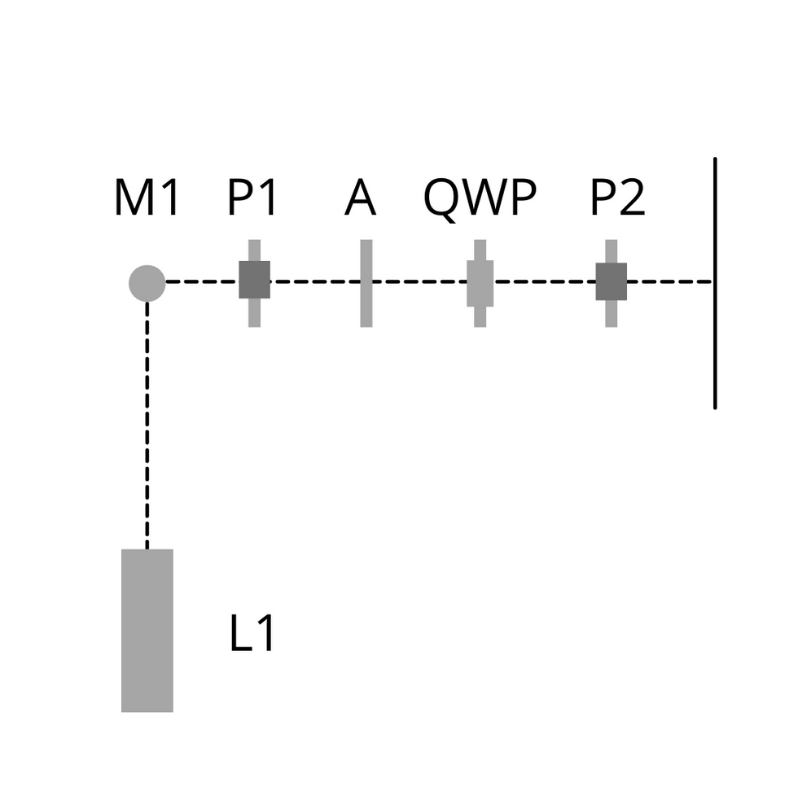
\includegraphics[width=0.31\textwidth]{E2}
  \end{center}
  \caption{Polarizers surrounding an aperture and a quarter waveplate. L1: laser, M1: mirror, P1: polarizer, A: aperture, HWP: quarter waveplate, P2: polarizer.}\label{E2}
\end{wrapfigure}
\large{\textbf{\S}}
After figuring out what a half waveplate did, it was not very difficult to complete my next objective: determine the use of a quarter waveplate and 3D glasses. I already knew half waveplates shifted by a half wavelength, so, logically, a quarter waveplate would shift by a quarter wavelength. Graphing this, however, made no sense because the phase shift between the components did not produce a linearly polarized wave, instead they produced a pattern that followed a helical pattern as they propagated. Never having heard of circularly polarized light, this representation made no sense to me, and I thought I was wrong in my assumption. Over and over again, I produced the same result in graphing it. I decided to keep with it and use it as my hypothesis. If I was correct, then the light passed through a QWP would not vary in intensity as it was passed through a linear polarizer. I confirmed my hypothesis with minimal difficulty.

As for the 3D glasses, I began by placing them in front of light polarized by P1 with aperture A closed to see if there was any change in intensity. With the front of the glasses pointing toward the incoming laser, I noticed that there was no change in intensity as I rotated the lenses along the optical axis. This effect very similar to what the QWP did, I noted, though it was not changing the polarization. The light remained linearly polarized. Placing the glasses in front of the QWP I noted that the right and left lenses of the glasses were opposite in their effect: the right lens would allow light through when rotated $-45^{\circ}$, and the left lens would allow through when rotated $45^{\circ}$. Based upon this, I hypothesized that the glasses must act as circular polarizers. Thinking I had arrived at a complete conjecture, I brought my results to Dr. Statman. I was partially correct; the lenses were indeed circular polarizers, but when flipping the lenses, they also acted as linear polarizers. Returning to the lab, I confirmed this to be true.

% --------------------------------------------------------------
\newpage
\noindent
\begin{wrapfigure}{r}{0.33\textwidth}
  \begin{center}
    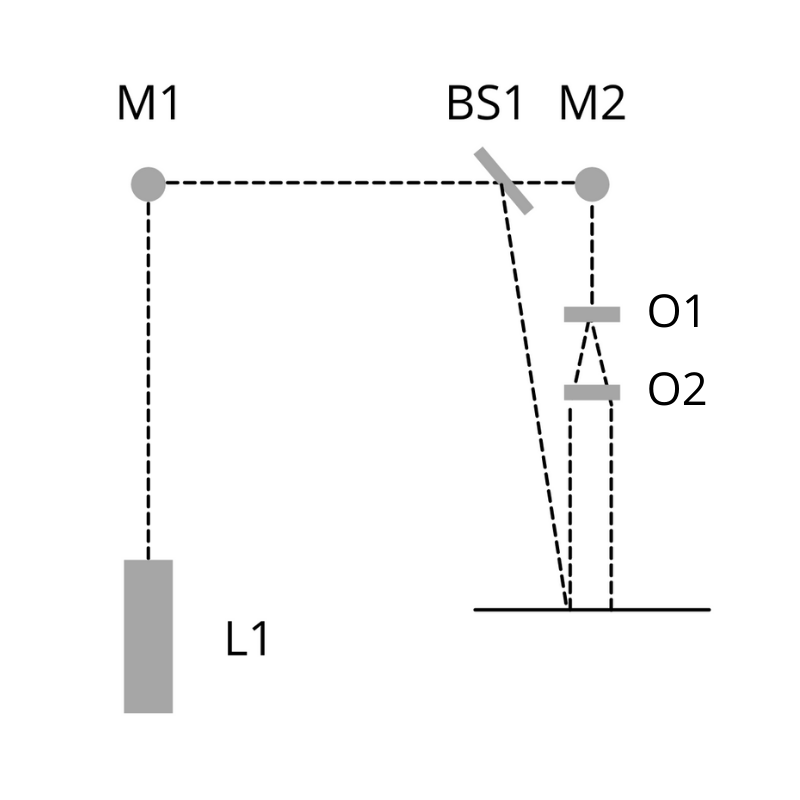
\includegraphics[width=0.31\textwidth]{E3}
  \end{center}
  \caption{Beam expander with split beam of original diameter for comparing. L1: laser, M1: mirror, BS1: beam splitter, M2: mirror, O1: diverging lens ($f=-10$cm), O2: converging lens ($f=30$cm).}\label{E3}
\end{wrapfigure}
\large{\textbf{\S}}
Prior to designing a beam expander, I was given three hints: the system must involve a diverging lens and a converging lens, their focal lengths must be aligned, and the magnification can be determined by the ration of their focal lengths, Eq.~\eqref{magnification}. I was told to achieve $5-10$ times magnification; however, I was only able to achieve $3$ times magnification because my access to lenses was limited. Knowing little about geometrical optics, I did not jump to using Eq.~\eqref{lensmakers}; instead, I tried different combinations of a diverging lens, O1, and a converging lens, O2. Out of curiosity, I tried a Galilean beam expander, in which two converging lenses are used, but I failed. Going back to the original plan, I tried to line up the focal lengths of O1 and O2 to be concurrent. It was not until I realized a negative focal length traces backwards from the diverged light that I knew how to create the beam expander; I saw a drawing on a nearby whiteboard of a similar beam expander, featuring a diverging lens followed by a converging lens. I set O1 stationary and moved O2 so that it was 20cm away from O1. This would allow O2's focal length to be concurrent with O2's. The beam passed through the diverging lens first, then the converging lens. Logically, it made sense that a diverging beam would be made parallel after passing through a converging lens if positioned appropriately. Using an index card to ensure the beams were parallel, I adjusted the lenses' relative positions until the beam remained a constant diameter as it reached the far field. After this was done, I positioned a beam splitter to direct part of the original beam onto the far field to compare the change in diameter. The beam's original diameter was 3mm, and the expanded beam came to approximately 9mm; with the ratio between O1 and O2 being 3, a 3 times expansion was indeed to be expected.

% --------------------------------------------------------------
\newpage
\noindent
\begin{wrapfigure}{r}{0.50\textwidth}
  \begin{center}
    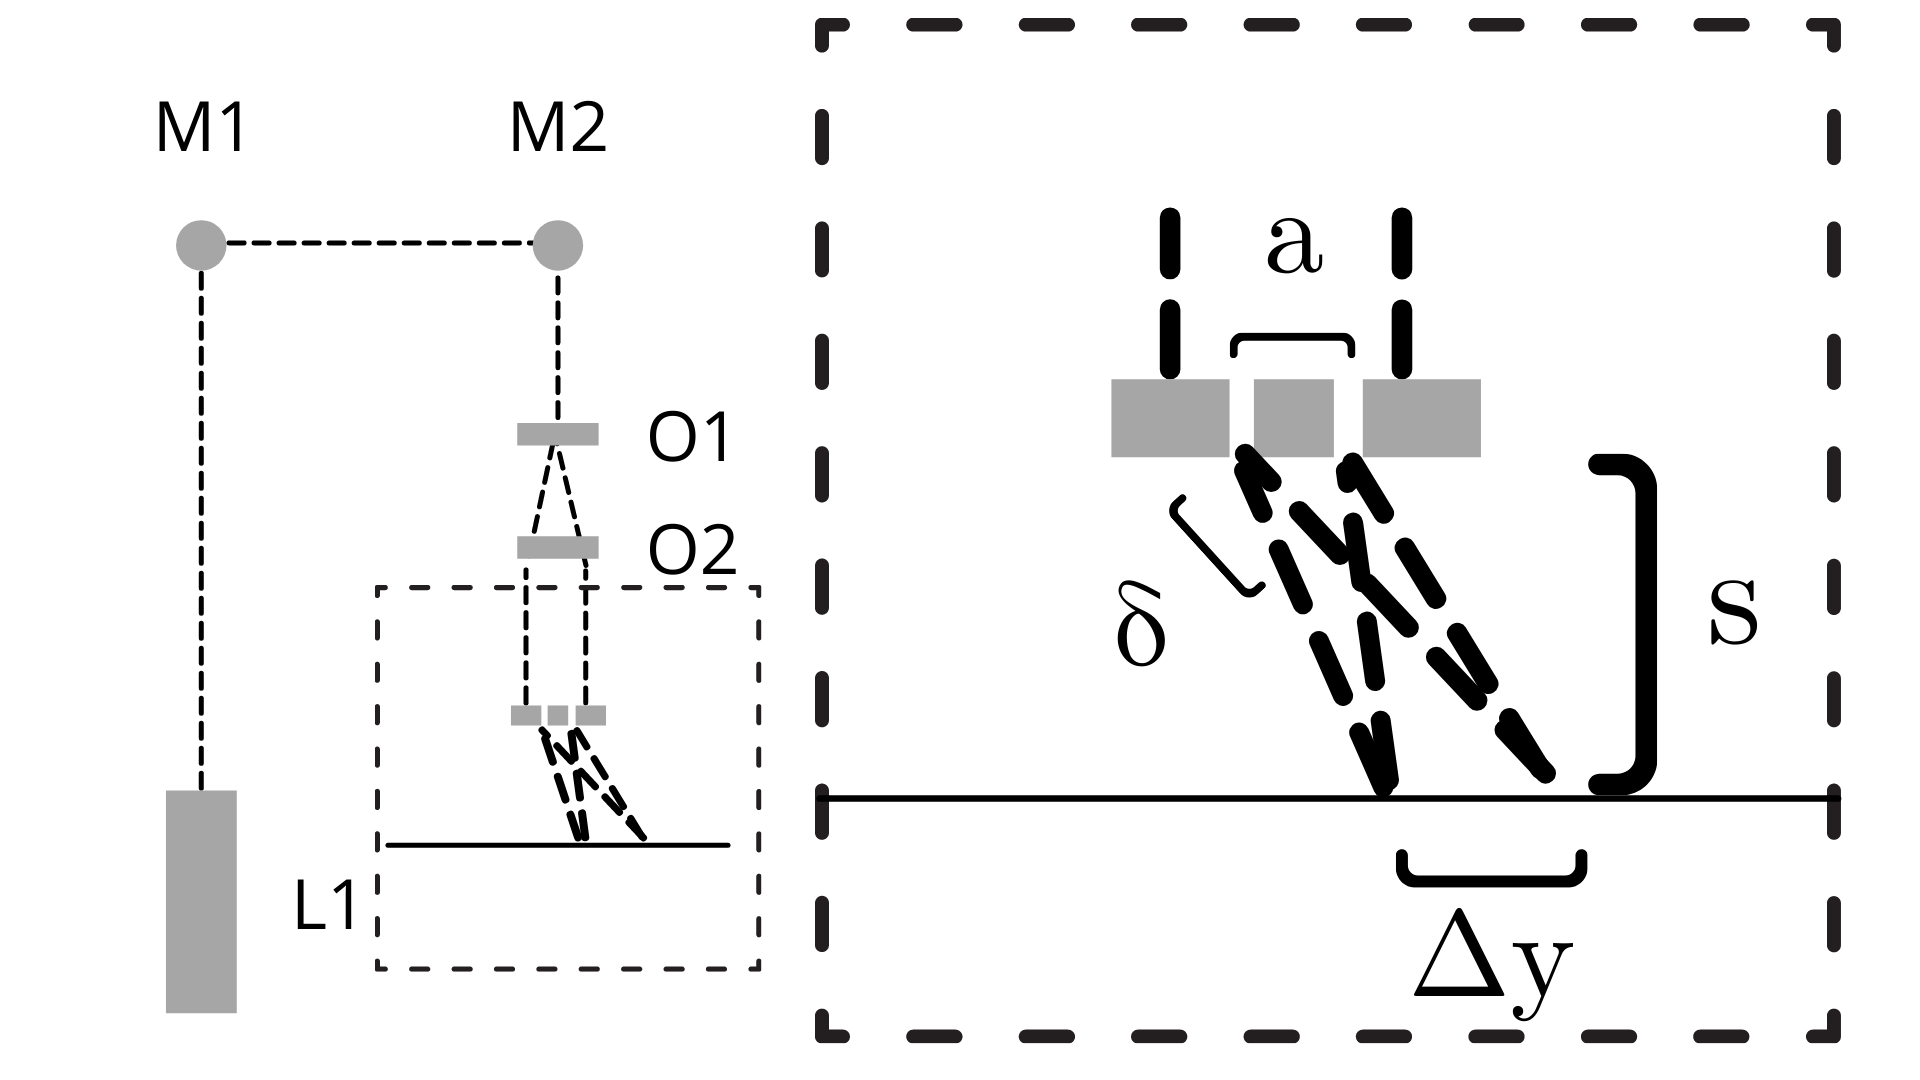
\includegraphics[width=0.48\textwidth]{E4.1}
  \end{center}
  \caption{Young's Double Slit Experiment and its geometrical features. L1: laser, M1: mirror, M2: mirror, O1: diverging lens, O2: converging lens.}\label{E4.1}
  \begin{center}
    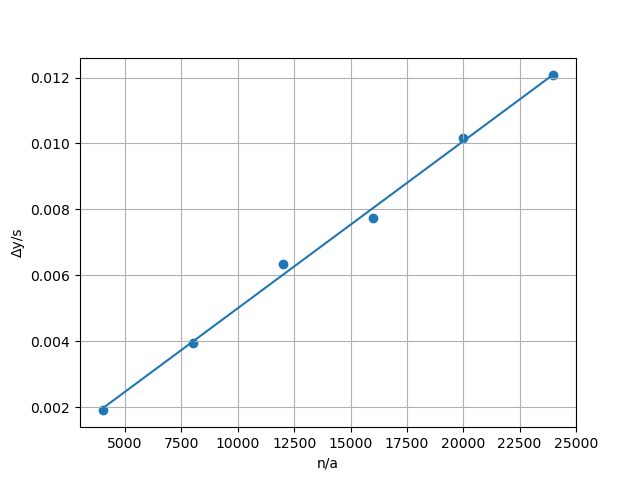
\includegraphics[width=0.48\textwidth]{E4.2}
  \end{center}
  \caption{Plotting $\frac{\Delta{y}}{s}$ versus $a^{-1}$ to arrive at a wavelength of $480$nm.}\label{E4.2}
\end{wrapfigure}
\large{\textbf{\S}}
Using Young's double slit experiment, seen in Fig.~\ref{E4.1}, I was able to calculate the wavelength of L1. The slit apparatus I used had four pairs of slits, two where $a=.25$mm and two where $a=.5$mm. At first, I took individual data points using Eq.~\eqref{wavelengthslitapprox}, measuring with a ruler, and averaged them to conclude that $\lambda=380$nm. This method proved to be inaccurate; for L1, $\lambda=488$nm!

I moved on to try to graph the slope. I took six data points of $[na^{-1}, \frac{\Delta{y}}{s}]$. Instead of leaving $n=1$, I decided to take measurments for different values of $n$. If I had not done so, I would have only had two data points because there are only two distinct values for $a$ in the slit apparatus. I created a program to graph the trendline given the data I had calculated. The resulting trendline had a slope of $\lambda=480$nm. Being within 8nm of the true wavelength, this method worked far better than the former.

% --------------------------------------------------------------
\newpage
\noindent
\begin{wrapfigure}{l}{.5\textwidth}
  \begin{center}
    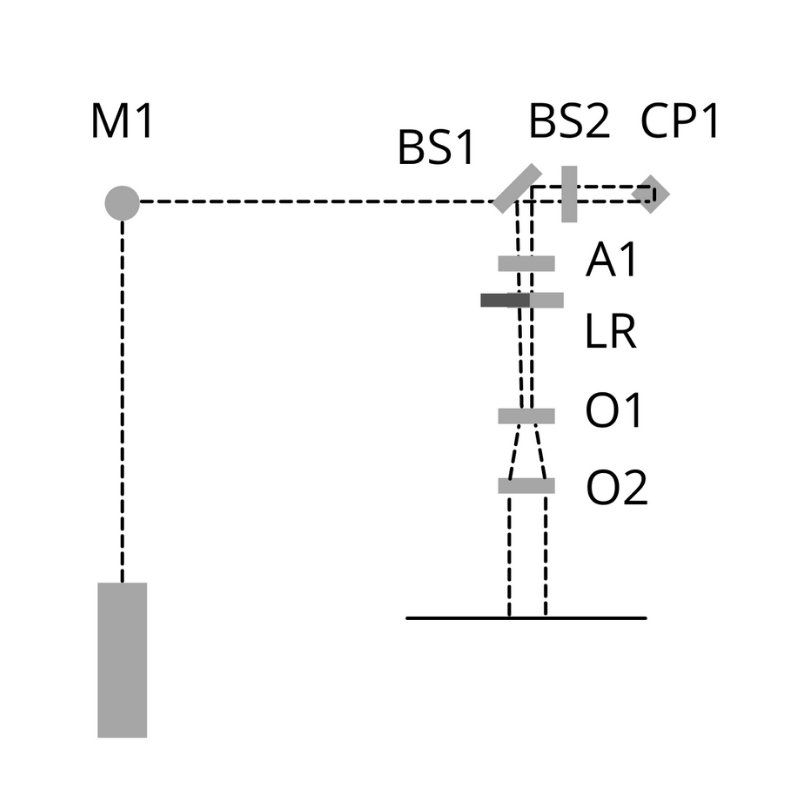
\includegraphics[width=0.48\textwidth]{E5}
  \end{center}
  \caption{Splitting a beam to be R/L polarized, interfered, then expanded. L1: laser, BS1: beam splitter, BS2: beam splitter, CP1: cubic prism, A1: aperture, LR: right/left circular polarizer, O1: diverging lens, O2: converging lens.}\label{E5}
\end{wrapfigure}
\large{\textbf{\S}}
To analyze the interference pattern between right and left circularly polarized light, I split a beam with a combination of a cubic prism and two beam splitters, shown in Fig.~\ref{E5}. After failing to align mirrrors close enough together to aim two nearly parallel beams into LR, I used this combination of BS1, BS2, and CP1 to produce nearly parallel beams. I ran into difficulty with the beam splitters reflecting back on themselves and traveling along the same path to the beam expander, causing unwanted interference, but it did not hinder the experiment. After being split, the beam passed through a sheet of right/left polarizing material, giving both beams the opposite polarizations. The beams traveled and interfered and were then expanded for analyzing.

Passing the expanded beam through a linear polarizer, I saw visible lines; however they would not move when I rotated the polarizer. Tweaking the setup to achieve closer parallel beams with the intention of producing more interference, the beams appeared the same as they did initially. Dr. Statman decided the visible lines were enough to move forward, though they would not move.

% --------------------------------------------------------------
\newpage
\noindent
\begin{wrapfigure}{r}{0.50\textwidth}
  \begin{center}
    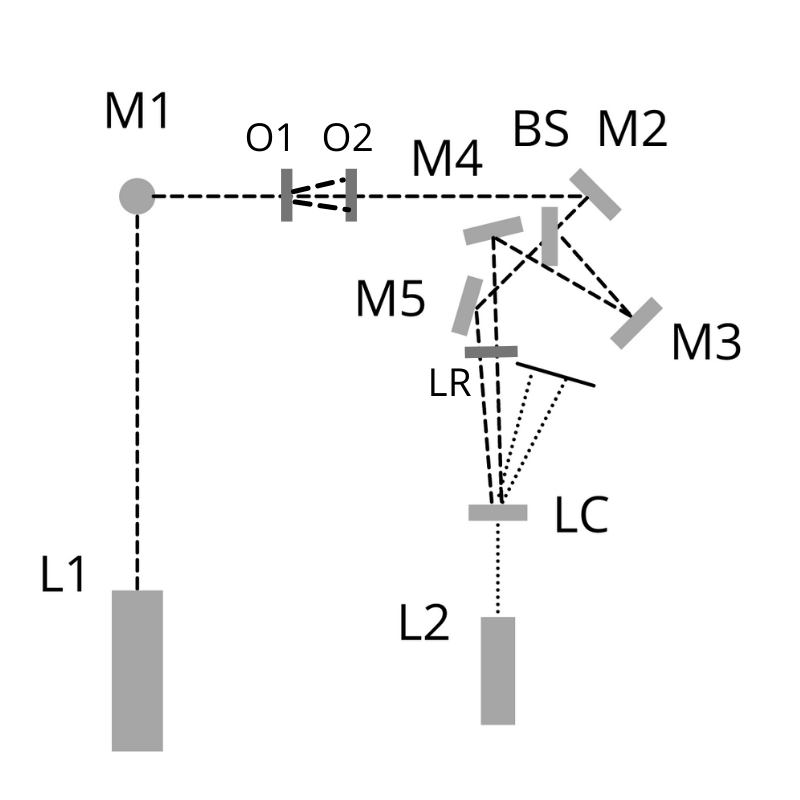
\includegraphics[width=0.48\textwidth]{E6.1}
  \end{center}
  \caption{First attempt at a vector hologram. L1: laser ($\lambda=488$nm), M(1, 2, 3, 4, 5): mirrors, O1 and O2: beam expander seen in Fig.~\ref{E3}, BS: beam splitter, LR: left/right polarizing material, LC: liquid crystal, L2: laser ($\lambda=488$nm).}\label{E6.1}
  \begin{center}
    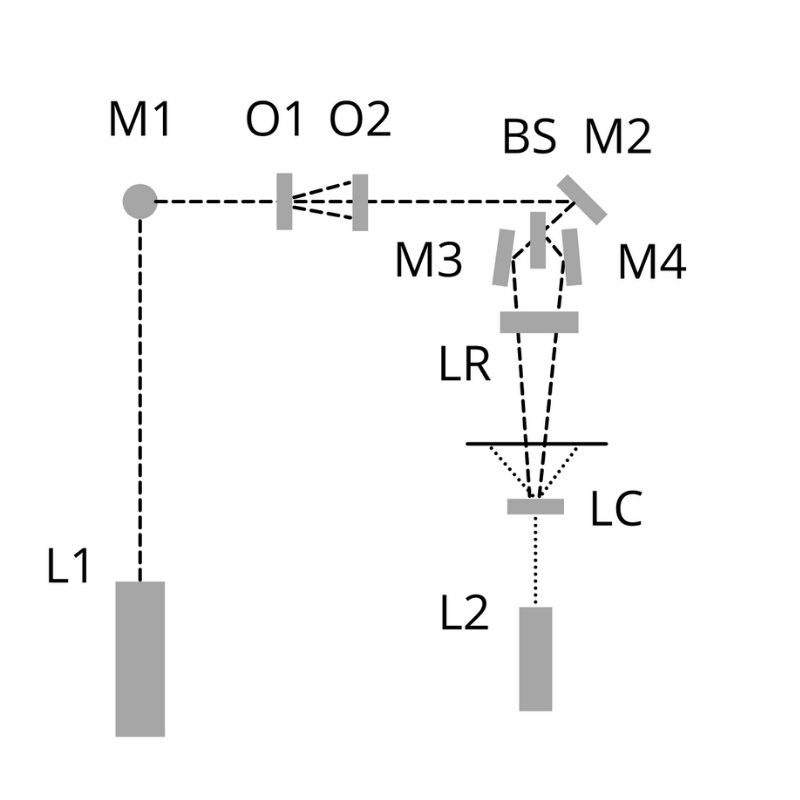
\includegraphics[width=0.48\textwidth]{E6.2}
  \end{center}
  \caption{Second attempt at a vector hologram with minimal path length difference. Components are the same as Fig.~\ref{E6.1}.}\label{E6.2}
\end{wrapfigure}
\large{\textbf{\S}}
As a sort of capstone, I started to work on constructing a vector hologram. I preserved some of the setup from the previous experiment in doing so. My first attempt, depicted in Fig.~\ref{E6.1}, shows an expanded beam being split to form nearly parallel beams. I expanded the beam so there would a larger diameter for the beams to cross paths and interfere. Just like the last experiment, these beams were oppositely polarized and interfered, but this time I directed them into a liquid crystal. If they were interfered well, directing L2 in the opposite direction into the liquid crystal would produce an image. No matter what I tried, I could not get this setup to work. I cleaned the lenses, tried to make the beams even more parallel, and tried crossing the beams' paths over a longer distance for optimal interference to no avail. Corresponding with Dr. Statman, he advised I reduce the difference in path length between the two lasers.

Fig.~\ref{E6.2} shows the revised setup with reduced path length. The problem with this setup was that, even though the path lengths were nearly identical, the intensities between both beams after passing through LR differed by nearly 80 percent. I ignored this, not knowing the consequences. When Dr. Statman reviewed my setup, he expressed just how great of an issue this was. The larger the difference in intensity, the less of a chance the beams would interfere effectively. Placing a neutral density filter between LR and LC, I achieved just under a 5 percent difference in intensity; however, I was still unable to see the expected row of dots from this vector hologram. Having worked on this inconclusive experiment for three weeks, we decided it was time to let the experiment go for this semester.

\subsection*{Discussion}
This independent study has prepared me well for future lab work by providing me experience in conducting, documenting, and presenting lab experiments. Although the level of complexity of the experiments may not surmount to that of an upperclassman, I feel that I will be able to conduct more experiments, and possibly research, in this field with more of an edge than my peers thanks to this invaluable experience.

Working with interference and polarization may be a pathway toward researching properties of electromagnetism to be used in digital communications. Additionally, as a computer scientist, I have always had an affinity toward this field of physics as an opportunity for developing various solutions.

Developing an understanding of the general concepts in optics has also pushed me to contribute to the Nim programming language to develop a library for computational optics. My hope is that this will allow others to conduct similar optics experiments in this cutting edge language without the overhead of forming their own models. As I continue education and research in this field, I will expand on this library.

I could not be any more grateful for the mentorship Dr. Statman has provided me this semester. The insight he gives and rigor he expects were instrumental in motivating my work. I look forward to collaborations to come in the following years.

\newpage

\begin{center}
  \large{\textbf{Bibliography}}
\end{center}

\printbibliography[heading=none]

\end{document}
